\documentclass[border=3pt]{standalone}
% Preâmbulo compartilhado pelos diagramas TikZ da aula 4 de Navegação (Representação de Mapas)
\usepackage[T1]{fontenc}
\usepackage[utf8]{inputenc}
\usepackage{lmodern}
\usepackage{amsmath}
\usepackage{xcolor}
\usepackage{tikz}
\usetikzlibrary{arrows.meta,angles,quotes,decorations.pathmorphing,decorations.pathreplacing,calc,
                positioning,shapes.geometric,shapes.misc,backgrounds,fit,
                math}

% Paleta (mesma dos SVGs originais)
\definecolor{dblue}{HTML}{2A5B8C}
\definecolor{dorange}{HTML}{B3541E}
\definecolor{dgreen}{HTML}{4A7C59}
\definecolor{dred}{HTML}{9C4B4B}
\definecolor{dcream}{HTML}{F4F1EA}
\definecolor{dshade}{HTML}{DDD7C9}

% Função gaussiana (não normalizada por padrão de escala visual)
\pgfmathdeclarefunction{gauss}{3}{%
  \pgfmathparse{1/(#3*sqrt(2*pi))*exp(-((#1-#2)^2)/(2*#3^2))}%
}

% Estilos comuns (prefixo d... para não colidir com chaves internas do pgf)
\tikzset{
  >={Stealth[length=2mm]},
  dguide/.style={gray!55, dashed, line width=0.4pt},
  daxis/.style={gray!60, line width=0.7pt, ->},
  dbody/.style={fill=black!3, draw=black!80, line width=1pt},
  dacc/.style={draw=dblue, line width=1pt},
  dlbl/.style={black!55, font=\small},
  dsub/.style={black!45, font=\footnotesize},
  dstate/.style={circle, draw=black!80, fill=dcream, line width=1pt,
                 minimum size=17mm, font=\large, inner sep=1pt},
  dobs/.style={circle, draw=black!80, fill=dshade, line width=1pt,
               minimum size=14mm, font=\large, inner sep=1pt},
  dbox/.style={rounded corners=2pt, draw=black!80, fill=dcream, line width=1pt,
               align=center, inner sep=6pt},
  dop/.style={circle, draw=black!80, fill=white, line width=1pt,
              minimum size=6mm, inner sep=0pt, font=\small},
  dtrans/.style={->, dblue, line width=1pt},
  dmeas/.style={->, dorange, line width=1pt},
  dcurve/.style={line width=1pt, dblue},
  dcurveb/.style={line width=1.4pt, dorange},
}

\begin{document}
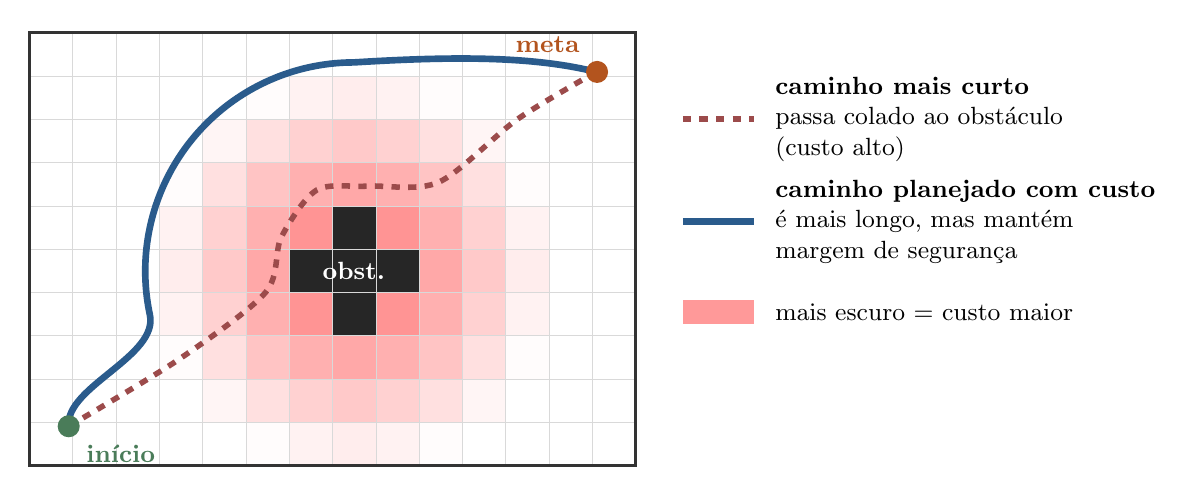
\begin{tikzpicture}[x=1cm,y=1cm]
\fill[red!0!white, draw=black!15, line width=0.2pt] (0.000,4.950) rectangle ++(0.55,0.55);
\fill[red!0!white, draw=black!15, line width=0.2pt] (0.000,4.400) rectangle ++(0.55,0.55);
\fill[red!0!white, draw=black!15, line width=0.2pt] (0.000,3.850) rectangle ++(0.55,0.55);
\fill[red!0!white, draw=black!15, line width=0.2pt] (0.000,3.300) rectangle ++(0.55,0.55);
\fill[red!0!white, draw=black!15, line width=0.2pt] (0.000,2.750) rectangle ++(0.55,0.55);
\fill[red!0!white, draw=black!15, line width=0.2pt] (0.000,2.200) rectangle ++(0.55,0.55);
\fill[red!0!white, draw=black!15, line width=0.2pt] (0.000,1.650) rectangle ++(0.55,0.55);
\fill[red!0!white, draw=black!15, line width=0.2pt] (0.000,1.100) rectangle ++(0.55,0.55);
\fill[red!0!white, draw=black!15, line width=0.2pt] (0.000,0.550) rectangle ++(0.55,0.55);
\fill[red!0!white, draw=black!15, line width=0.2pt] (0.000,0.000) rectangle ++(0.55,0.55);
\fill[red!0!white, draw=black!15, line width=0.2pt] (0.550,4.950) rectangle ++(0.55,0.55);
\fill[red!0!white, draw=black!15, line width=0.2pt] (0.550,4.400) rectangle ++(0.55,0.55);
\fill[red!0!white, draw=black!15, line width=0.2pt] (0.550,3.850) rectangle ++(0.55,0.55);
\fill[red!0!white, draw=black!15, line width=0.2pt] (0.550,3.300) rectangle ++(0.55,0.55);
\fill[red!0!white, draw=black!15, line width=0.2pt] (0.550,2.750) rectangle ++(0.55,0.55);
\fill[red!0!white, draw=black!15, line width=0.2pt] (0.550,2.200) rectangle ++(0.55,0.55);
\fill[red!0!white, draw=black!15, line width=0.2pt] (0.550,1.650) rectangle ++(0.55,0.55);
\fill[red!0!white, draw=black!15, line width=0.2pt] (0.550,1.100) rectangle ++(0.55,0.55);
\fill[red!0!white, draw=black!15, line width=0.2pt] (0.550,0.550) rectangle ++(0.55,0.55);
\fill[red!0!white, draw=black!15, line width=0.2pt] (0.550,0.000) rectangle ++(0.55,0.55);
\fill[red!0!white, draw=black!15, line width=0.2pt] (1.100,4.950) rectangle ++(0.55,0.55);
\fill[red!0!white, draw=black!15, line width=0.2pt] (1.100,4.400) rectangle ++(0.55,0.55);
\fill[red!0!white, draw=black!15, line width=0.2pt] (1.100,3.850) rectangle ++(0.55,0.55);
\fill[red!0!white, draw=black!15, line width=0.2pt] (1.100,3.300) rectangle ++(0.55,0.55);
\fill[red!0!white, draw=black!15, line width=0.2pt] (1.100,2.750) rectangle ++(0.55,0.55);
\fill[red!0!white, draw=black!15, line width=0.2pt] (1.100,2.200) rectangle ++(0.55,0.55);
\fill[red!0!white, draw=black!15, line width=0.2pt] (1.100,1.650) rectangle ++(0.55,0.55);
\fill[red!0!white, draw=black!15, line width=0.2pt] (1.100,1.100) rectangle ++(0.55,0.55);
\fill[red!0!white, draw=black!15, line width=0.2pt] (1.100,0.550) rectangle ++(0.55,0.55);
\fill[red!0!white, draw=black!15, line width=0.2pt] (1.100,0.000) rectangle ++(0.55,0.55);
\fill[red!0!white, draw=black!15, line width=0.2pt] (1.650,4.950) rectangle ++(0.55,0.55);
\fill[red!0!white, draw=black!15, line width=0.2pt] (1.650,4.400) rectangle ++(0.55,0.55);
\fill[red!0!white, draw=black!15, line width=0.2pt] (1.650,3.850) rectangle ++(0.55,0.55);
\fill[red!1!white, draw=black!15, line width=0.2pt] (1.650,3.300) rectangle ++(0.55,0.55);
\fill[red!5!white, draw=black!15, line width=0.2pt] (1.650,2.750) rectangle ++(0.55,0.55);
\fill[red!7!white, draw=black!15, line width=0.2pt] (1.650,2.200) rectangle ++(0.55,0.55);
\fill[red!5!white, draw=black!15, line width=0.2pt] (1.650,1.650) rectangle ++(0.55,0.55);
\fill[red!1!white, draw=black!15, line width=0.2pt] (1.650,1.100) rectangle ++(0.55,0.55);
\fill[red!0!white, draw=black!15, line width=0.2pt] (1.650,0.550) rectangle ++(0.55,0.55);
\fill[red!0!white, draw=black!15, line width=0.2pt] (1.650,0.000) rectangle ++(0.55,0.55);
\fill[red!0!white, draw=black!15, line width=0.2pt] (2.200,4.950) rectangle ++(0.55,0.55);
\fill[red!0!white, draw=black!15, line width=0.2pt] (2.200,4.400) rectangle ++(0.55,0.55);
\fill[red!4!white, draw=black!15, line width=0.2pt] (2.200,3.850) rectangle ++(0.55,0.55);
\fill[red!12!white, draw=black!15, line width=0.2pt] (2.200,3.300) rectangle ++(0.55,0.55);
\fill[red!18!white, draw=black!15, line width=0.2pt] (2.200,2.750) rectangle ++(0.55,0.55);
\fill[red!21!white, draw=black!15, line width=0.2pt] (2.200,2.200) rectangle ++(0.55,0.55);
\fill[red!18!white, draw=black!15, line width=0.2pt] (2.200,1.650) rectangle ++(0.55,0.55);
\fill[red!12!white, draw=black!15, line width=0.2pt] (2.200,1.100) rectangle ++(0.55,0.55);
\fill[red!4!white, draw=black!15, line width=0.2pt] (2.200,0.550) rectangle ++(0.55,0.55);
\fill[red!0!white, draw=black!15, line width=0.2pt] (2.200,0.000) rectangle ++(0.55,0.55);
\fill[red!0!white, draw=black!15, line width=0.2pt] (2.750,4.950) rectangle ++(0.55,0.55);
\fill[red!1!white, draw=black!15, line width=0.2pt] (2.750,4.400) rectangle ++(0.55,0.55);
\fill[red!12!white, draw=black!15, line width=0.2pt] (2.750,3.850) rectangle ++(0.55,0.55);
\fill[red!23!white, draw=black!15, line width=0.2pt] (2.750,3.300) rectangle ++(0.55,0.55);
\fill[red!31!white, draw=black!15, line width=0.2pt] (2.750,2.750) rectangle ++(0.55,0.55);
\fill[red!34!white, draw=black!15, line width=0.2pt] (2.750,2.200) rectangle ++(0.55,0.55);
\fill[red!31!white, draw=black!15, line width=0.2pt] (2.750,1.650) rectangle ++(0.55,0.55);
\fill[red!23!white, draw=black!15, line width=0.2pt] (2.750,1.100) rectangle ++(0.55,0.55);
\fill[red!12!white, draw=black!15, line width=0.2pt] (2.750,0.550) rectangle ++(0.55,0.55);
\fill[red!1!white, draw=black!15, line width=0.2pt] (2.750,0.000) rectangle ++(0.55,0.55);
\fill[red!0!white, draw=black!15, line width=0.2pt] (3.300,4.950) rectangle ++(0.55,0.55);
\fill[red!5!white, draw=black!15, line width=0.2pt] (3.300,4.400) rectangle ++(0.55,0.55);
\fill[red!18!white, draw=black!15, line width=0.2pt] (3.300,3.850) rectangle ++(0.55,0.55);
\fill[red!31!white, draw=black!15, line width=0.2pt] (3.300,3.300) rectangle ++(0.55,0.55);
\fill[red!42!white, draw=black!15, line width=0.2pt] (3.300,2.750) rectangle ++(0.55,0.55);
\fill[black!85, draw=black!15, line width=0.2pt] (3.300,2.200) rectangle ++(0.55,0.55);
\fill[red!42!white, draw=black!15, line width=0.2pt] (3.300,1.650) rectangle ++(0.55,0.55);
\fill[red!31!white, draw=black!15, line width=0.2pt] (3.300,1.100) rectangle ++(0.55,0.55);
\fill[red!18!white, draw=black!15, line width=0.2pt] (3.300,0.550) rectangle ++(0.55,0.55);
\fill[red!5!white, draw=black!15, line width=0.2pt] (3.300,0.000) rectangle ++(0.55,0.55);
\fill[red!0!white, draw=black!15, line width=0.2pt] (3.850,4.950) rectangle ++(0.55,0.55);
\fill[red!7!white, draw=black!15, line width=0.2pt] (3.850,4.400) rectangle ++(0.55,0.55);
\fill[red!21!white, draw=black!15, line width=0.2pt] (3.850,3.850) rectangle ++(0.55,0.55);
\fill[red!34!white, draw=black!15, line width=0.2pt] (3.850,3.300) rectangle ++(0.55,0.55);
\fill[black!85, draw=black!15, line width=0.2pt] (3.850,2.750) rectangle ++(0.55,0.55);
\fill[black!85, draw=black!15, line width=0.2pt] (3.850,2.200) rectangle ++(0.55,0.55);
\fill[black!85, draw=black!15, line width=0.2pt] (3.850,1.650) rectangle ++(0.55,0.55);
\fill[red!34!white, draw=black!15, line width=0.2pt] (3.850,1.100) rectangle ++(0.55,0.55);
\fill[red!21!white, draw=black!15, line width=0.2pt] (3.850,0.550) rectangle ++(0.55,0.55);
\fill[red!7!white, draw=black!15, line width=0.2pt] (3.850,0.000) rectangle ++(0.55,0.55);
\fill[red!0!white, draw=black!15, line width=0.2pt] (4.400,4.950) rectangle ++(0.55,0.55);
\fill[red!5!white, draw=black!15, line width=0.2pt] (4.400,4.400) rectangle ++(0.55,0.55);
\fill[red!18!white, draw=black!15, line width=0.2pt] (4.400,3.850) rectangle ++(0.55,0.55);
\fill[red!31!white, draw=black!15, line width=0.2pt] (4.400,3.300) rectangle ++(0.55,0.55);
\fill[red!42!white, draw=black!15, line width=0.2pt] (4.400,2.750) rectangle ++(0.55,0.55);
\fill[black!85, draw=black!15, line width=0.2pt] (4.400,2.200) rectangle ++(0.55,0.55);
\fill[red!42!white, draw=black!15, line width=0.2pt] (4.400,1.650) rectangle ++(0.55,0.55);
\fill[red!31!white, draw=black!15, line width=0.2pt] (4.400,1.100) rectangle ++(0.55,0.55);
\fill[red!18!white, draw=black!15, line width=0.2pt] (4.400,0.550) rectangle ++(0.55,0.55);
\fill[red!5!white, draw=black!15, line width=0.2pt] (4.400,0.000) rectangle ++(0.55,0.55);
\fill[red!0!white, draw=black!15, line width=0.2pt] (4.950,4.950) rectangle ++(0.55,0.55);
\fill[red!1!white, draw=black!15, line width=0.2pt] (4.950,4.400) rectangle ++(0.55,0.55);
\fill[red!12!white, draw=black!15, line width=0.2pt] (4.950,3.850) rectangle ++(0.55,0.55);
\fill[red!23!white, draw=black!15, line width=0.2pt] (4.950,3.300) rectangle ++(0.55,0.55);
\fill[red!31!white, draw=black!15, line width=0.2pt] (4.950,2.750) rectangle ++(0.55,0.55);
\fill[red!34!white, draw=black!15, line width=0.2pt] (4.950,2.200) rectangle ++(0.55,0.55);
\fill[red!31!white, draw=black!15, line width=0.2pt] (4.950,1.650) rectangle ++(0.55,0.55);
\fill[red!23!white, draw=black!15, line width=0.2pt] (4.950,1.100) rectangle ++(0.55,0.55);
\fill[red!12!white, draw=black!15, line width=0.2pt] (4.950,0.550) rectangle ++(0.55,0.55);
\fill[red!1!white, draw=black!15, line width=0.2pt] (4.950,0.000) rectangle ++(0.55,0.55);
\fill[red!0!white, draw=black!15, line width=0.2pt] (5.500,4.950) rectangle ++(0.55,0.55);
\fill[red!0!white, draw=black!15, line width=0.2pt] (5.500,4.400) rectangle ++(0.55,0.55);
\fill[red!4!white, draw=black!15, line width=0.2pt] (5.500,3.850) rectangle ++(0.55,0.55);
\fill[red!12!white, draw=black!15, line width=0.2pt] (5.500,3.300) rectangle ++(0.55,0.55);
\fill[red!18!white, draw=black!15, line width=0.2pt] (5.500,2.750) rectangle ++(0.55,0.55);
\fill[red!21!white, draw=black!15, line width=0.2pt] (5.500,2.200) rectangle ++(0.55,0.55);
\fill[red!18!white, draw=black!15, line width=0.2pt] (5.500,1.650) rectangle ++(0.55,0.55);
\fill[red!12!white, draw=black!15, line width=0.2pt] (5.500,1.100) rectangle ++(0.55,0.55);
\fill[red!4!white, draw=black!15, line width=0.2pt] (5.500,0.550) rectangle ++(0.55,0.55);
\fill[red!0!white, draw=black!15, line width=0.2pt] (5.500,0.000) rectangle ++(0.55,0.55);
\fill[red!0!white, draw=black!15, line width=0.2pt] (6.050,4.950) rectangle ++(0.55,0.55);
\fill[red!0!white, draw=black!15, line width=0.2pt] (6.050,4.400) rectangle ++(0.55,0.55);
\fill[red!0!white, draw=black!15, line width=0.2pt] (6.050,3.850) rectangle ++(0.55,0.55);
\fill[red!1!white, draw=black!15, line width=0.2pt] (6.050,3.300) rectangle ++(0.55,0.55);
\fill[red!5!white, draw=black!15, line width=0.2pt] (6.050,2.750) rectangle ++(0.55,0.55);
\fill[red!7!white, draw=black!15, line width=0.2pt] (6.050,2.200) rectangle ++(0.55,0.55);
\fill[red!5!white, draw=black!15, line width=0.2pt] (6.050,1.650) rectangle ++(0.55,0.55);
\fill[red!1!white, draw=black!15, line width=0.2pt] (6.050,1.100) rectangle ++(0.55,0.55);
\fill[red!0!white, draw=black!15, line width=0.2pt] (6.050,0.550) rectangle ++(0.55,0.55);
\fill[red!0!white, draw=black!15, line width=0.2pt] (6.050,0.000) rectangle ++(0.55,0.55);
\fill[red!0!white, draw=black!15, line width=0.2pt] (6.600,4.950) rectangle ++(0.55,0.55);
\fill[red!0!white, draw=black!15, line width=0.2pt] (6.600,4.400) rectangle ++(0.55,0.55);
\fill[red!0!white, draw=black!15, line width=0.2pt] (6.600,3.850) rectangle ++(0.55,0.55);
\fill[red!0!white, draw=black!15, line width=0.2pt] (6.600,3.300) rectangle ++(0.55,0.55);
\fill[red!0!white, draw=black!15, line width=0.2pt] (6.600,2.750) rectangle ++(0.55,0.55);
\fill[red!0!white, draw=black!15, line width=0.2pt] (6.600,2.200) rectangle ++(0.55,0.55);
\fill[red!0!white, draw=black!15, line width=0.2pt] (6.600,1.650) rectangle ++(0.55,0.55);
\fill[red!0!white, draw=black!15, line width=0.2pt] (6.600,1.100) rectangle ++(0.55,0.55);
\fill[red!0!white, draw=black!15, line width=0.2pt] (6.600,0.550) rectangle ++(0.55,0.55);
\fill[red!0!white, draw=black!15, line width=0.2pt] (6.600,0.000) rectangle ++(0.55,0.55);
\fill[red!0!white, draw=black!15, line width=0.2pt] (7.150,4.950) rectangle ++(0.55,0.55);
\fill[red!0!white, draw=black!15, line width=0.2pt] (7.150,4.400) rectangle ++(0.55,0.55);
\fill[red!0!white, draw=black!15, line width=0.2pt] (7.150,3.850) rectangle ++(0.55,0.55);
\fill[red!0!white, draw=black!15, line width=0.2pt] (7.150,3.300) rectangle ++(0.55,0.55);
\fill[red!0!white, draw=black!15, line width=0.2pt] (7.150,2.750) rectangle ++(0.55,0.55);
\fill[red!0!white, draw=black!15, line width=0.2pt] (7.150,2.200) rectangle ++(0.55,0.55);
\fill[red!0!white, draw=black!15, line width=0.2pt] (7.150,1.650) rectangle ++(0.55,0.55);
\fill[red!0!white, draw=black!15, line width=0.2pt] (7.150,1.100) rectangle ++(0.55,0.55);
\fill[red!0!white, draw=black!15, line width=0.2pt] (7.150,0.550) rectangle ++(0.55,0.55);
\fill[red!0!white, draw=black!15, line width=0.2pt] (7.150,0.000) rectangle ++(0.55,0.55);
\draw[black!80, line width=1.2pt] (0,0) rectangle (7.70,5.50);
\draw[dred, line width=2pt, dashed] plot[smooth] coordinates {(0.50,0.50) (1.9,1.35) (3.0,2.2) (3.2,2.9) (3.65,3.5) (4.3,3.55) (5.2,3.6) (6.2,4.4) (7.2,5.0)};
\draw[dblue, line width=2.4pt] (0.50,0.50) .. controls (0.45,1.0) and (1.65,1.39) .. (1.53,1.92) arc[start angle=192, end angle=90, radius=2.65] .. controls (5.4,5.2) and (6.4,5.2) .. (7.2,5.0);
\fill[dgreen] (0.50,0.50) circle (0.14); \node[dgreen, font=\small\bfseries, anchor=north west] at (0.60,0.38) {início};
\fill[dorange] (7.21,5.00) circle (0.14); \node[dorange, font=\small\bfseries, anchor=south east] at (7.11,5.12) {meta};
\node[white, font=\small\bfseries] at (4.12,2.48) {obst.};
\draw[dred, line width=2pt, dashed] (8.30,4.4) -- (9.20,4.4); \node[anchor=west, font=\small, align=left] at (9.35,4.4) {\textbf{caminho mais curto}\\ passa colado ao obstáculo\\ (custo alto)};
\draw[dblue, line width=2.4pt] (8.30,3.1) -- (9.20,3.1); \node[anchor=west, font=\small, align=left] at (9.35,3.1) {\textbf{caminho planejado com custo}\\ é mais longo, mas mantém\\ margem de segurança};
\fill[red!40!white] (8.30,1.8) rectangle ++(0.9,0.3); \node[anchor=west, font=\small, align=left] at (9.35,1.95) {mais escuro = custo maior};
\end{tikzpicture}
\end{document}
